\section{مدل تفصیلی ظرفیت \lr{Diffusion}}
\subsection{مساحت کف و محیط کناره‌ها}
در بخش \secnum{۲.۳.۳} کتاب، ظرفیت پیوند \lr{Source} و \lr{Body} از دو سهم
کف و کناره محاسبه می‌شود. برای ناحیه مستطیلی با عرض \(W\) و امتداد بیرون
کانال \(D_{\mathrm{diff}}\)، مساحت و محیط برابرند با
\begin{equation}
 A=WD_{\mathrm{diff}},\qquad P=2W+2D_{\mathrm{diff}}.
 \label{eq:cv-diffusion-geometry}
\end{equation}
کتاب برای امتداد هندسی نماد \(D\) را به کار می‌برد. در این جزوه، پسوند
\(\mathrm{diff}\) آن را از نام پایانه \lr{Drain} مشخص می‌کند.
برای یک لبه مجاور کانال، طول لبه روبه‌روی \lr{Gate} برابر \(P_g=W\) و طول
باقی کناره‌ها \(P_{\mathrm{non}}=W+2D_{\mathrm{diff}}\) است.
جمع این دو، محیط کل \(P\) می‌شود \cite[شکل \secnum{۲.۱۲}]{weste}.

در مدل دوضریبی رابطه \secnum{۲.۱۶} کتاب، برای \lr{Source} داریم
\begin{equation}
 C_{SB}=A_SC_{jbs}+P_SC_{jbssw}.
 \label{eq:cv-two-coeff-junction}
\end{equation}
\(A_S\) و \(P_S\) به‌ترتیب مساحت و محیط \lr{Source} هستند.
\(C_{jbs}\) ظرفیت بر واحد سطح کف با واحدی مانند
\unit{\femto\farad\per\micro\metre\squared} و \(C_{jbssw}\) ظرفیت بر واحد طول
کناره با واحدی مانند \unit{\femto\farad\per\micro\metre} است.
هر دو حاصل‌ضرب واحد \unit{\femto\farad} دارند.

در مدل دارای ضریب مستقل برای لبه روبه‌روی کانال، جمع به صورت
\begin{equation}
 C_{SB}(V_R)=A_SC_A(V_R)+P_{\mathrm{non},S}c_{\mathrm{sw}}(V_R)
 +P_{g,S}c_{\mathrm{swg}}(V_R)
 \label{eq:cv-three-coeff-junction}
\end{equation}
نوشته می‌شود. \(C_A\) ضریب سطحی و \(c_{\mathrm{sw}},c_{\mathrm{swg}}\)
ضرایب طولی دو نوع کناره هستند. حروف کوچک در ضرایب طولی، واحد متفاوت را
در این جزوه روشن می‌کنند. همه طول‌های محیط میان دو دسته تقسیم شده‌اند.

کتاب در توضیح فناوری دارای \lr{Shallow Trench Isolation} یا \lr{STI}،
اهمیت متفاوت کناره عایق‌شده و کناره روبه‌روی کانال را توضیح می‌دهد
\cite[صفحه ۷۲]{weste}. برای \lr{Drain} نیز همین ساختار با مساحت \(A_D\)،
محیط‌های مربوط و ولتاژ پیوند \lr{Drain}-\lr{Body} به کار می‌رود.
پارامترهای \lr{nMOS} و \lr{pMOS} از فناوری همان افزاره گرفته می‌شوند.

\subsection{وابستگی به بایاس و معنای توان منفی}
\(V_R\ge0\) را بزرگی بایاس معکوس پیوند می‌نامیم. برای \lr{nMOS}، در سمت
\lr{Source}، \(V_R=V_S-V_B\) و در سمت \lr{Drain}، \(V_R=V_D-V_B\) است.
برای \lr{pMOS} با \lr{Body} پرپتانسیل‌تر، این بزرگی‌ها به‌ترتیب
\(V_B-V_S\) و \(V_B-V_D\) هستند. استفاده از بزرگی معکوس، دامنه ولتاژ فرمول
را برای هر دو نوع افزاره روشن می‌کند.

با افزایش بایاس معکوس، ناحیه \lr{Depletion} پهن‌تر می‌شود و ظرفیت کاهش می‌یابد.
رابطه سطحی کتاب چنین است
\begin{equation}
 C_A(V_R)=C_J\left(1+\frac{V_R}{\psi_0}\right)^{-M_J}
 =\frac{C_J}{(1+V_R/\psi_0)^{M_J}}.
 \label{eq:cv-area-bias}
\end{equation}
\(C_J\) ضریب سطحی در بایاس صفر، \(\psi_0\) پتانسیل داخلی پیوند و \(M_J\)
ضریب \lr{Junction Grading} است. کتاب برای \(M_J\) حدود \num{0.33} تا
\num{0.5} ذکر می‌کند \cite[رابطه \secnum{۲.۱۷}]{weste}.
داخل پرانتز بی‌بعد است، زیرا دو ولتاژ بر هم تقسیم شده‌اند.
توان منفی یعنی معکوس توان مثبت. اگر \(V_R\) افزایش یابد، مخرج برای \(M_J>0\)
بزرگ‌تر و ظرفیت کوچک‌تر می‌شود. در \(V_R=0\)، ضریب ظرفیت دقیقاً \(C_J\) است.

دو نوع ضریب کناره نیز با پارامترهای خود از روابط مشابه به دست می‌آیند
\begin{align}
 c_{\mathrm{sw}}(V_R)
 &=C_{JSW}\left(1+\frac{V_R}{\psi_{SW}}\right)^{-M_{JSW}},\notag\\
 c_{\mathrm{swg}}(V_R)
 &=C_{JSWG}\left(1+\frac{V_R}{\psi_{SWG}}\right)^{-M_{JSWG}}.
 \label{eq:cv-sidewall-bias}
\end{align}
در چاپ رابطه \secnum{۲.۲۰} کتاب، ضریب جلوی جمله سمت کانال با نماد
\(C_{JSW}\) دیده می‌شود، اما مثال \secnum{۲.۲} برای این سمت، پارامتر مستقل
\(C_{JSWG}\) می‌دهد. در \eqref{eq:cv-sidewall-bias} نام مستقل مطابق همان
مثال حفظ شده است. مدل انتخاب‌شده باید برای هر لبه ضریب مشخص داشته باشد.

این روابط برای بایاس معکوس یا صفر در نظر گرفته شده‌اند.
در بایاس مستقیم، مدل پیوند و هدایت آن به تحلیل مناسب آن شرایط نیاز دارد.
مثلاً جای‌گذاری بدون توجه به علامت بایاس \lr{pMOS} می‌تواند پایه توان کسری
را از دامنه معتبر مدل خارج کند.

\subsection{\lr{Thermal Voltage}، پتانسیل داخلی و لگاریتم طبیعی}
کتاب پتانسیل داخلی پیوند را به \lr{Doping} و دما مرتبط می‌کند
\begin{equation}
 \psi_0=v_T\ln\left(\frac{N_AN_D}{n_i^2}\right),\qquad
 v_T=\frac{kT}{q}.
 \label{eq:cv-built-in}
\end{equation}
\(N_A\) و \(N_D\) غلظت \lr{Acceptor} و \lr{Donor}، و \(n_i\) غلظت
حامل ذاتی‌اند. هر سه باید با واحد یکسان، مانند \unit{\per\centi\metre\cubed}،
جای‌گذاری شوند تا نسبت داخل لگاریتم بی‌بعد شود.
\(v_T\) در این رابطه \lr{Thermal Voltage} است.
\lr{Threshold Voltage} ترانزیستور در بخش‌های پیشین با \(V_{tn}\) یا
\(V_{tp}\) مشخص شده است \cite[رابطه \secnum{۲.۱۸}]{weste}.

\(T\) دمای مطلق بر حسب \unit{\kelvin}، \(k\) ثابت \lr{Boltzmann} و \(q\)
بزرگی بار الکترون است. با ثابت‌های گرد‌شده کتاب در \(T=\qty{300}{\kelvin}\)، داریم
\begin{equation*}
 v_T=\frac{(1.380\times10^{-23})(300)}{1.602\times10^{-19}}
 \,\unit{\volt}\approx\qty{0.02584}{\volt}\approx\qty{26}{\milli\volt}.
\end{equation*}
واحد \(kT\) انرژی و واحد \(q\) بار است. نسبت انرژی به بار، ولتاژ می‌شود.
برای تبدیل دمای سلسیوس، \(T\) بر حسب کلوین از افزودن \num{273.15} به مقدار
سلسیوس به دست می‌آید. مقدار \qty{300}{\kelvin} تقریب دمای اتاق در داده کتاب است.

\(\ln\) لگاریتم طبیعی با پایه \(e\approx\num{2.718}\) است.
اگر \(y=\ln x\)، آنگاه \(e^y=x\). برای محاسبه دستی می‌توان از
\(\ln(ab)=\ln a+\ln b\) و \(\ln(10^n)=n\ln10\) استفاده کرد.
برای غلظت‌های فرضی \(N_A=10^{16}\)، \(N_D=10^{17}\) و مقدار کتاب
\(n_i=1.45\times10^{10}\)، همگی در \unit{\per\centi\metre\cubed}، داریم
\begin{align*}
 \frac{N_AN_D}{n_i^2}
 &=\frac{10^{33}}{(1.45)^2\times10^{20}}
 \approx4.756\times10^{12},\\
 \ln(4.756\times10^{12})&=\ln4.756+12\ln10\approx29.19,\\
 \psi_0&\approx(0.02584)(29.19)\,\unit{\volt}\approx\qty{0.754}{\volt}.
\end{align*}
غلظت‌های فرضی این محاسبه برای توضیح لگاریتم انتخاب شده‌اند.
در مثال کتاب، مقدار \(\psi_0\) مستقیماً داده شده و همان مقدار استفاده می‌شود.

\subsection{حل مرحله‌ای مثال \texorpdfstring{\secnum{۲.۲}}{۲.۲} کتاب}
مثال \secnum{۲.۲}، ظرفیت \lr{Drain} یک \lr{nMOS} دارای \lr{Contact} را
در فناوری \qty{65}{\nano\metre} می‌خواهد. اندازه \(\lambda\)، عرض و امتداد
ناحیه به صورت زیر داده شده‌اند.
\[
 \lambda=\qty{25}{\nano\metre},\qquad
 W=4\lambda=\qty{0.1}{\micro\metre},\qquad
 D_{\mathrm{diff}}=5\lambda=\qty{0.125}{\micro\metre}.
\]
\lr{Body} به زمین وصل است و \(V_D\) ابتدا صفر و سپس \qty{1}{\volt} می‌شود
\cite[صفحه ۷۳]{weste}.
پارامترهای مثال چنین‌اند
\begin{align*}
 C_J&=\qty{1.2}{\femto\farad\per\micro\metre\squared},
 &M_J&=0.33,\\
 C_{JSW}&=\qty{0.1}{\femto\farad\per\micro\metre},
 &C_{JSWG}&=\qty{0.36}{\femto\farad\per\micro\metre},\\
 M_{JSW}&=M_{JSWG}=0.10,
 &\psi_0&=\qty{0.7}{\volt}.
\end{align*}
محاسبه کتاب برای کناره‌ها نیز از همین پتانسیل \qty{0.7}{\volt} استفاده می‌کند.
برای تطبیق آن، \(\psi_{SW}=\psi_{SWG}=\psi_0\) می‌گیریم.
هندسه ابتدا به صورت مستقل محاسبه می‌شود
\begin{align}
 A_D&=(0.1)(0.125)=\qty{0.0125}{\micro\metre\squared},\notag\\
 P_D&=2(0.1)+2(0.125)=\qty{0.45}{\micro\metre},\notag\\
 P_g&=W=\qty{0.1}{\micro\metre},\qquad
 P_{\mathrm{non}}=P_D-P_g=\qty{0.35}{\micro\metre}.
 \label{eq:cv-book-geometry}
\end{align}
در بایاس صفر، هر عامل \((1+V_R/\psi)^{-M}\) برابر یک است. با ضرب جداگانه هر
ضریب در هندسه متناظر، ظرفیت می‌شود
\begin{align*}
 C_{DB}(0)
 &=(0.0125)(1.2)+(0.35)(0.1)+(0.1)(0.36)\quad\unit{\femto\farad}\\
 &=(0.015+0.035+0.036)\,\unit{\femto\farad}
 =\qty{0.086}{\femto\farad}.
\end{align*}
در خط اول، واحد طول یا مساحت هر عدد هندسی، همان واحد داده‌شده در
\eqref{eq:cv-book-geometry} است و در ضرب با ضریب مناسب حذف می‌شود.
مجموع دو سهم کناره در این مثال \qty{0.071}{\femto\farad} است.

در \(V_D=\qty{1}{\volt}\)، بایاس معکوس \(V_R=\qty{1}{\volt}\) می‌شود.
عامل مشترک داخل پرانتز را \(r=1+1/0.7\approx2.42857\) می‌نامیم.
سهم کف در \(r^{-0.33}\) و سهم کناره‌ها در \(r^{-0.10}\) ضرب می‌شود، پس
\begin{align*}
 C_{DB}(1)
 &=0.015r^{-0.33}+0.071r^{-0.10}\quad\unit{\femto\farad}\\
 &\approx\qty{0.0762}{\femto\farad}\approx\qty{0.076}{\femto\farad}.
\end{align*}
برای محاسبه با ماشین‌حساب، ابتدا \(r\)، سپس \(r^{0.33}\) و \(r^{0.10}\)
را می‌یابیم و هر ضریب را بر توان مثبت مربوط تقسیم می‌کنیم.
کاهش ظرفیت با افزایش بایاس معکوس، با تفسیر پهن‌شدن \lr{Depletion} سازگار است.

کتاب برای تخمین دستی میانگین دو سر گذار را استفاده می‌کند
\begin{equation*}
 C_{DB,\mathrm{ends}}\approx\frac{0.086+0.076}{2}
 =\qty{0.081}{\femto\farad}.
\end{equation*}
این عدد، بازتولید تقریب مثال مرجع است. برای مقایسه، می‌توان معادل دقیق‌تر از
نظر بار همین تابع غیرخطی را با \eqref{eq:cv-charge-equivalent} محاسبه کرد.
برای هر مؤلفه \(C_a(1+V/\psi)^{-M}\) با \(M\ne1\)، انتگرال از صفر تا
\(V_{DD}\) به صورت
\begin{equation}
 \Delta Q=C_a\frac{\psi}{1-M}
 \left[\left(1+\frac{V_{DD}}{\psi}\right)^{1-M}-1\right]
 \label{eq:cv-junction-integral}
\end{equation}
درمی‌آید. عامل \(\psi\) از تبدیل متغیر \(u=1+V/\psi\) و
\(dV=\psi\,du\) حاصل می‌شود. با انتگرال توان \(u^{-M}\)، توان جدید
\(1-M\) و ضریب تقسیم بر \(1-M\) به دست می‌آیند.
جمع این رابطه برای سهم کف و دو کناره، سپس تقسیم بر \qty{1}{\volt}، ظرفیت
معادل بر پایه تغییر بار را می‌دهد. برای مقایسه عددی، با نگه‌داشتن ارقام میانی،
\(C_{\mathrm{eff},Q}\approx\qty{0.08023}{\femto\farad}\) و میانگین دو سر
گردنشده \(C_{\mathrm{ends}}\approx\qty{0.08108}{\femto\farad}\) می‌شود.
میانگین دو سر در این مثال حدود \num{1.1} درصد بیشتر است.
این محاسبه تکمیلی، دقت تقریب دستی را برای همین تابع و بازه می‌سنجد.

\subsection{هندسه \lr{Isolated}، \lr{Shared} و \lr{Merged}}
شکل \secnum{۲.۸} کتاب سه شکل اتصال دو ترانزیستور سری را نشان می‌دهد.
در \lr{Isolated Diffusion}، هر ترانزیستور ناحیه دارای \lr{Contact} خود را دارد
و دو ناحیه با سیم به هم وصل می‌شوند. در \lr{Shared Diffusion}، یک ناحیه مشترک
دارای \lr{Contact} میان دو \lr{Gate} قرار می‌گیرد.
در \lr{Merged Diffusion}، همان اتصال داخلی با ناحیه پیوسته بدون \lr{Contact}
ساخته می‌شود. شکل \ref{fig:cv-layout-types} فقط ناحیه داخلی مرتبط را نشان می‌دهد.

\begin{figure}[ht]
\centering
\begin{latin}
\PersianMathDigits
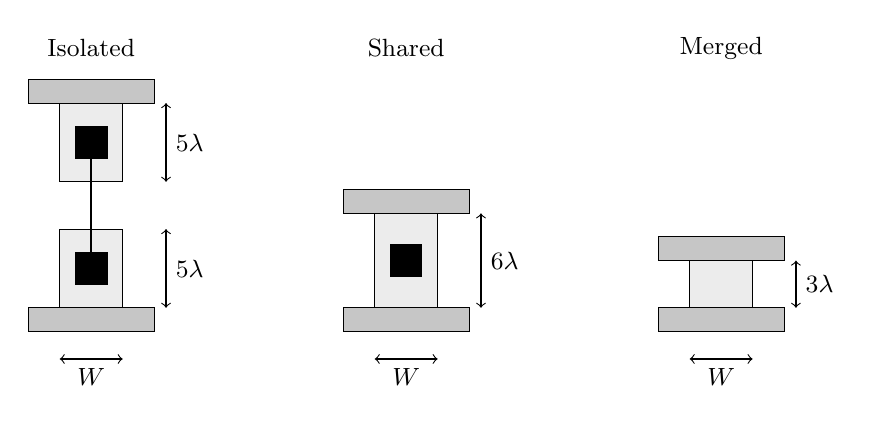
\begin{tikzpicture}[x=1cm,y=1cm,font=\small]
\node at (1,3.3) {Isolated};
\draw[fill=gray!15] (0.6,0) rectangle (1.4,1);
\draw[fill=gray!15] (0.6,1.6) rectangle (1.4,2.6);
\draw[fill=black] (0.8,0.3) rectangle (1.2,0.7);
\draw[fill=black] (0.8,1.9) rectangle (1.2,2.3);
\draw[thick] (1,0.5)--(1,2.1);
\draw[fill=gray!45] (0.2,-0.3) rectangle (1.8,0);
\draw[fill=gray!45] (0.2,2.6) rectangle (1.8,2.9);
\draw[<->] (1.95,0)--(1.95,1) node[midway,right] {$5\lambda$};
\draw[<->] (1.95,1.6)--(1.95,2.6) node[midway,right] {$5\lambda$};
\node at (5,3.3) {Shared};
\draw[fill=gray!15] (4.6,0) rectangle (5.4,1.2);
\draw[fill=black] (4.8,0.4) rectangle (5.2,0.8);
\draw[fill=gray!45] (4.2,-0.3) rectangle (5.8,0);
\draw[fill=gray!45] (4.2,1.2) rectangle (5.8,1.5);
\draw[<->] (5.95,0)--(5.95,1.2) node[midway,right] {$6\lambda$};
\node at (9,3.3) {Merged};
\draw[fill=gray!15] (8.6,0) rectangle (9.4,0.6);
\draw[fill=gray!45] (8.2,-0.3) rectangle (9.8,0);
\draw[fill=gray!45] (8.2,0.6) rectangle (9.8,0.9);
\draw[<->] (9.95,0)--(9.95,0.6) node[midway,right] {$3\lambda$};
\foreach \x in {1,5,9}{
 \draw[<->] (\x-0.4,-0.65)--(\x+0.4,-0.65) node[midway,below] {$W$};
}
\end{tikzpicture}
\end{latin}
\caption{بازترسیم آموزشی ناحیه داخلی دو ترانزیستور سری با هندسه شکل
\secnum{۲.۸} کتاب. نوارهای پهن تیره \lr{Gate}، مربع‌های سیاه \lr{Contact}
و مستطیل روشن \lr{Diffusion} است. خط میان دو \lr{Contact} حالت اول، اتصال
سیمی را نشان می‌دهد \cite{weste}.}
\label{fig:cv-layout-types}
\end{figure}

با \(W=4\lambda\)، \(\lambda=\qty{0.025}{\micro\metre}\) و پارامترهای
بایاس صفر مثال کتاب، می‌توان سهم پیوندی اتصال داخلی را مقایسه کرد.
برای دو ناحیه جدا، مساحت‌ها و کناره‌ها جمع می‌شوند. برای ناحیه مشترک یا
ادغام‌شده میان دو \lr{Gate}، دو لبه روبه‌روی کانال داریم، پس \(P_g=2W\)
و \(P_{\mathrm{non}}=2D_{\mathrm{diff}}\) می‌شود.
نتایج در جدول \ref{tab:cv-layout-area} آمده‌اند.

\begin{table}[ht]
\centering
\caption{مقایسه محاسبه‌شده فقط برای ظرفیت پیوندی گره داخلی در هندسه آموزشی شکل
\ref{fig:cv-layout-types} و بایاس صفر.}
\label{tab:cv-layout-area}
\begin{tabular}{ccccc}
\toprule
نوع & \(A\;(\unit{\micro\metre\squared})\) &
\(P_{\mathrm{non}}\;(\unit{\micro\metre})\) & \(P_g\;(\unit{\micro\metre})\) &
\(C_j\;(\unit{\femto\farad})\)\\
\midrule
\lr{Isolated}، دو ناحیه & \(0.025\) & \(0.70\) & \(0.20\) & \(0.172\)\\
\lr{Shared}، یک ناحیه & \(0.015\) & \(0.30\) & \(0.20\) & \(0.120\)\\
\lr{Merged}، یک ناحیه & \(0.0075\) & \(0.15\) & \(0.20\) & \(0.096\)\\
\bottomrule
\end{tabular}
\end{table}
برای نمونه، محاسبه سطر \lr{Shared} چنین است.
\[
 C_j=0.015(1.2)+0.30(0.1)+0.20(0.36)=\qty{0.120}{\femto\farad}.
\]
سهم لبه‌های روبه‌روی کانال با این تغییر ثابت مانده، اما سهم کف و کناره‌های
دیگر کاهش یافته است. در مدل کامل، ظرفیت‌های \lr{Gate} و سیم متصل به همین گره
نیز با قرارداد خود افزوده می‌شوند.

یک ناحیه فیزیکی مشترک، یک بار در محاسبه مستقیم هندسه گره شمارش می‌شود.
اگر مشخصه هندسی در \lr{Netlist} میان دو ترانزیستور تقسیم شود، مجموع سهم‌های
اختصاص‌یافته باید با همان ناحیه فیزیکی و قرارداد مدل سازگار باشد.
\lr{Gate Overlap} هر لبه نیز سهم جداگانه مربوط به همان \lr{Gate} است.
کاهش هندسه باید قواعد ساخت و نیاز اتصال را برآورده کند.
کتاب به ظرفیت و مقاومت زیاد \lr{Diffusion} اشاره می‌کند و کوچک‌نگه‌داشتن
آن را برای گره‌های متغیر توصیه می‌کند \cite[صفحه ۷۳]{weste}.

\subsection{تمرین‌های پاسخ‌دار \lr{Diffusion Capacitance}}
\textbf{تمرین ۸.} ناحیه‌ای فرضی با \(W=\qty{0.2}{\micro\metre}\) و
\(D_{\mathrm{diff}}=\qty{0.15}{\micro\metre}\) فقط یک لبه مجاور کانال دارد.
مساحت و دو محیط چیست؟ هندسه و ظرفیت با ضرایب بایاس صفر مثال کتاب
از محاسبات زیر به دست می‌آیند.
\[
 \begin{aligned}
 A&=0.2(0.15)=\qty{0.03}{\micro\metre\squared},&
 P_g&=\qty{0.2}{\micro\metre},\\
 P_{\mathrm{non}}&=0.2+2(0.15)=\qty{0.5}{\micro\metre},\\
 C_j&=0.03(1.2)+0.5(0.1)+0.2(0.36)=\qty{0.158}{\femto\farad}.
 \end{aligned}
\]

\textbf{تمرین ۹.} برای پیوند فرضی \(\psi=\qty{0.8}{\volt}\)، \(M=0.5\)
و بایاس \(V_R=\qty{0.8}{\volt}\)، نسبت ظرفیت به مقدار بایاس صفر چیست؟
\[
 (1+0.8/0.8)^{-0.5}=\frac{1}{\sqrt2}\approx0.707.
\]
پس ظرفیت حدود ۷۱ درصد مقدار بایاس صفر است.

\textbf{تمرین ۱۰.} در \lr{pMOS}، \(V_B=\qty{1.2}{\volt}\) و
\(V_D=\qty{0.2}{\volt}\) باشد. بزرگی بایاس معکوس پیوند \lr{Drain} چیست؟
\[
 V_R=V_B-V_D=\qty{1}{\volt}.
\]
برای جای‌گذاری باید پارامترهای پیوند
\lr{pMOS} همان فناوری نیز معلوم باشند.

\textbf{تمرین ۱۱.} در مدل مثال کتاب، آیا دوبرابرکردن عرض با ثابت‌ماندن
\(D_{\mathrm{diff}}\) همه سهم‌های ظرفیت پیوند را دقیقاً دو برابر می‌کند؟
مساحت \(WD_{\mathrm{diff}}\) و لبه \(P_g=W\) دو برابر می‌شوند.
اما \(P_{\mathrm{non}}=W+2D_{\mathrm{diff}}\) یک سهم ثابت دارد.
برای نمونه، از \(W=0.1\) به \(0.2\) و \(D_{\mathrm{diff}}=0.125\)، همگی
در \unit{\micro\metre}، ظرفیت بایاس صفر از \qty{0.086}{\femto\farad}
به \(0.025(1.2)+0.45(0.1)+0.2(0.36)=\qty{0.147}{\femto\farad}\) می‌رسد.
این نتیجه، علت تقریبی‌بودن تناسب ظرفیت \lr{Diffusion} با عرض را نشان می‌دهد.

\textbf{تمرین ۱۲.} در مثال بار خروجی \eqref{eq:cv-load-example}، اگر
ظرفیت پیوندی مشترک از هندسه دقیق محاسبه شده باشد، چگونه مدل‌ها را جمع کنیم؟
برای همان ناحیه، مقدار دقیق جای سهم ساده عرضی مربوط به آن ناحیه قرار می‌گیرد.
ظرفیت‌های ورودی مراحل بعد و سیم، هر کدام یک بار افزوده می‌شوند.
اگر ضریب مؤثر ورودی از قبل \lr{Overlap} را پوشش دهد، همان سهم در مدل ورودی
محسوب شده است. هدف، تهیه فهرست سهم‌های فیزیکی و مدل انتخاب‌شده برای هر سهم است.

\subsection{انتخاب سطح مدل در مسئله‌های درس}
وقتی مسئله ضریب بر واحد عرض می‌دهد، مدل ساده با همان ضریب و عرض به کار می‌رود.
وقتی ناحیه کاری و \(C_0\) و ضرایب هم‌پوشانی داده می‌شوند، مؤلفه‌های ذاتی و
\lr{Overlap} جدا محاسبه و سپس در پایانه مربوط جمع می‌شوند.
وقتی مساحت، محیط و ضرایب پیوند داده می‌شوند، مدل هندسی وابسته به بایاس به کار می‌رود.
در گذار بزرگ، تعریف ظرفیت مؤثر و مسیر ولتاژ نیز مشخص می‌شود.
این ترتیب انتخاب مدل، نتیجه را به داده‌ها، واحدها و شرایط مسئله متصل نگه می‌دارد.
\clearpage
